%-------------------------------------------------------------------------
\section{Experiments and Results}  \label{Sec:Experiments}
We test our DeepPRT method against different animated objects: We animate a \textit{Pirate Head} and a \textit{Fish} object using a blendshape model and apply physically-based deformations to animate a \textit{Cloth} object.
\\
The mesh resolution of the objects is $256 \times 256$. However, for the Fish object we increase the resolution to $512 \times 512$ to avoid reconstruction artifacts (see figure \ref{Fig: Fish Reconstruction})
% FIGURE (Fish Resampling)
\begin{figure}[H]
  \centering
    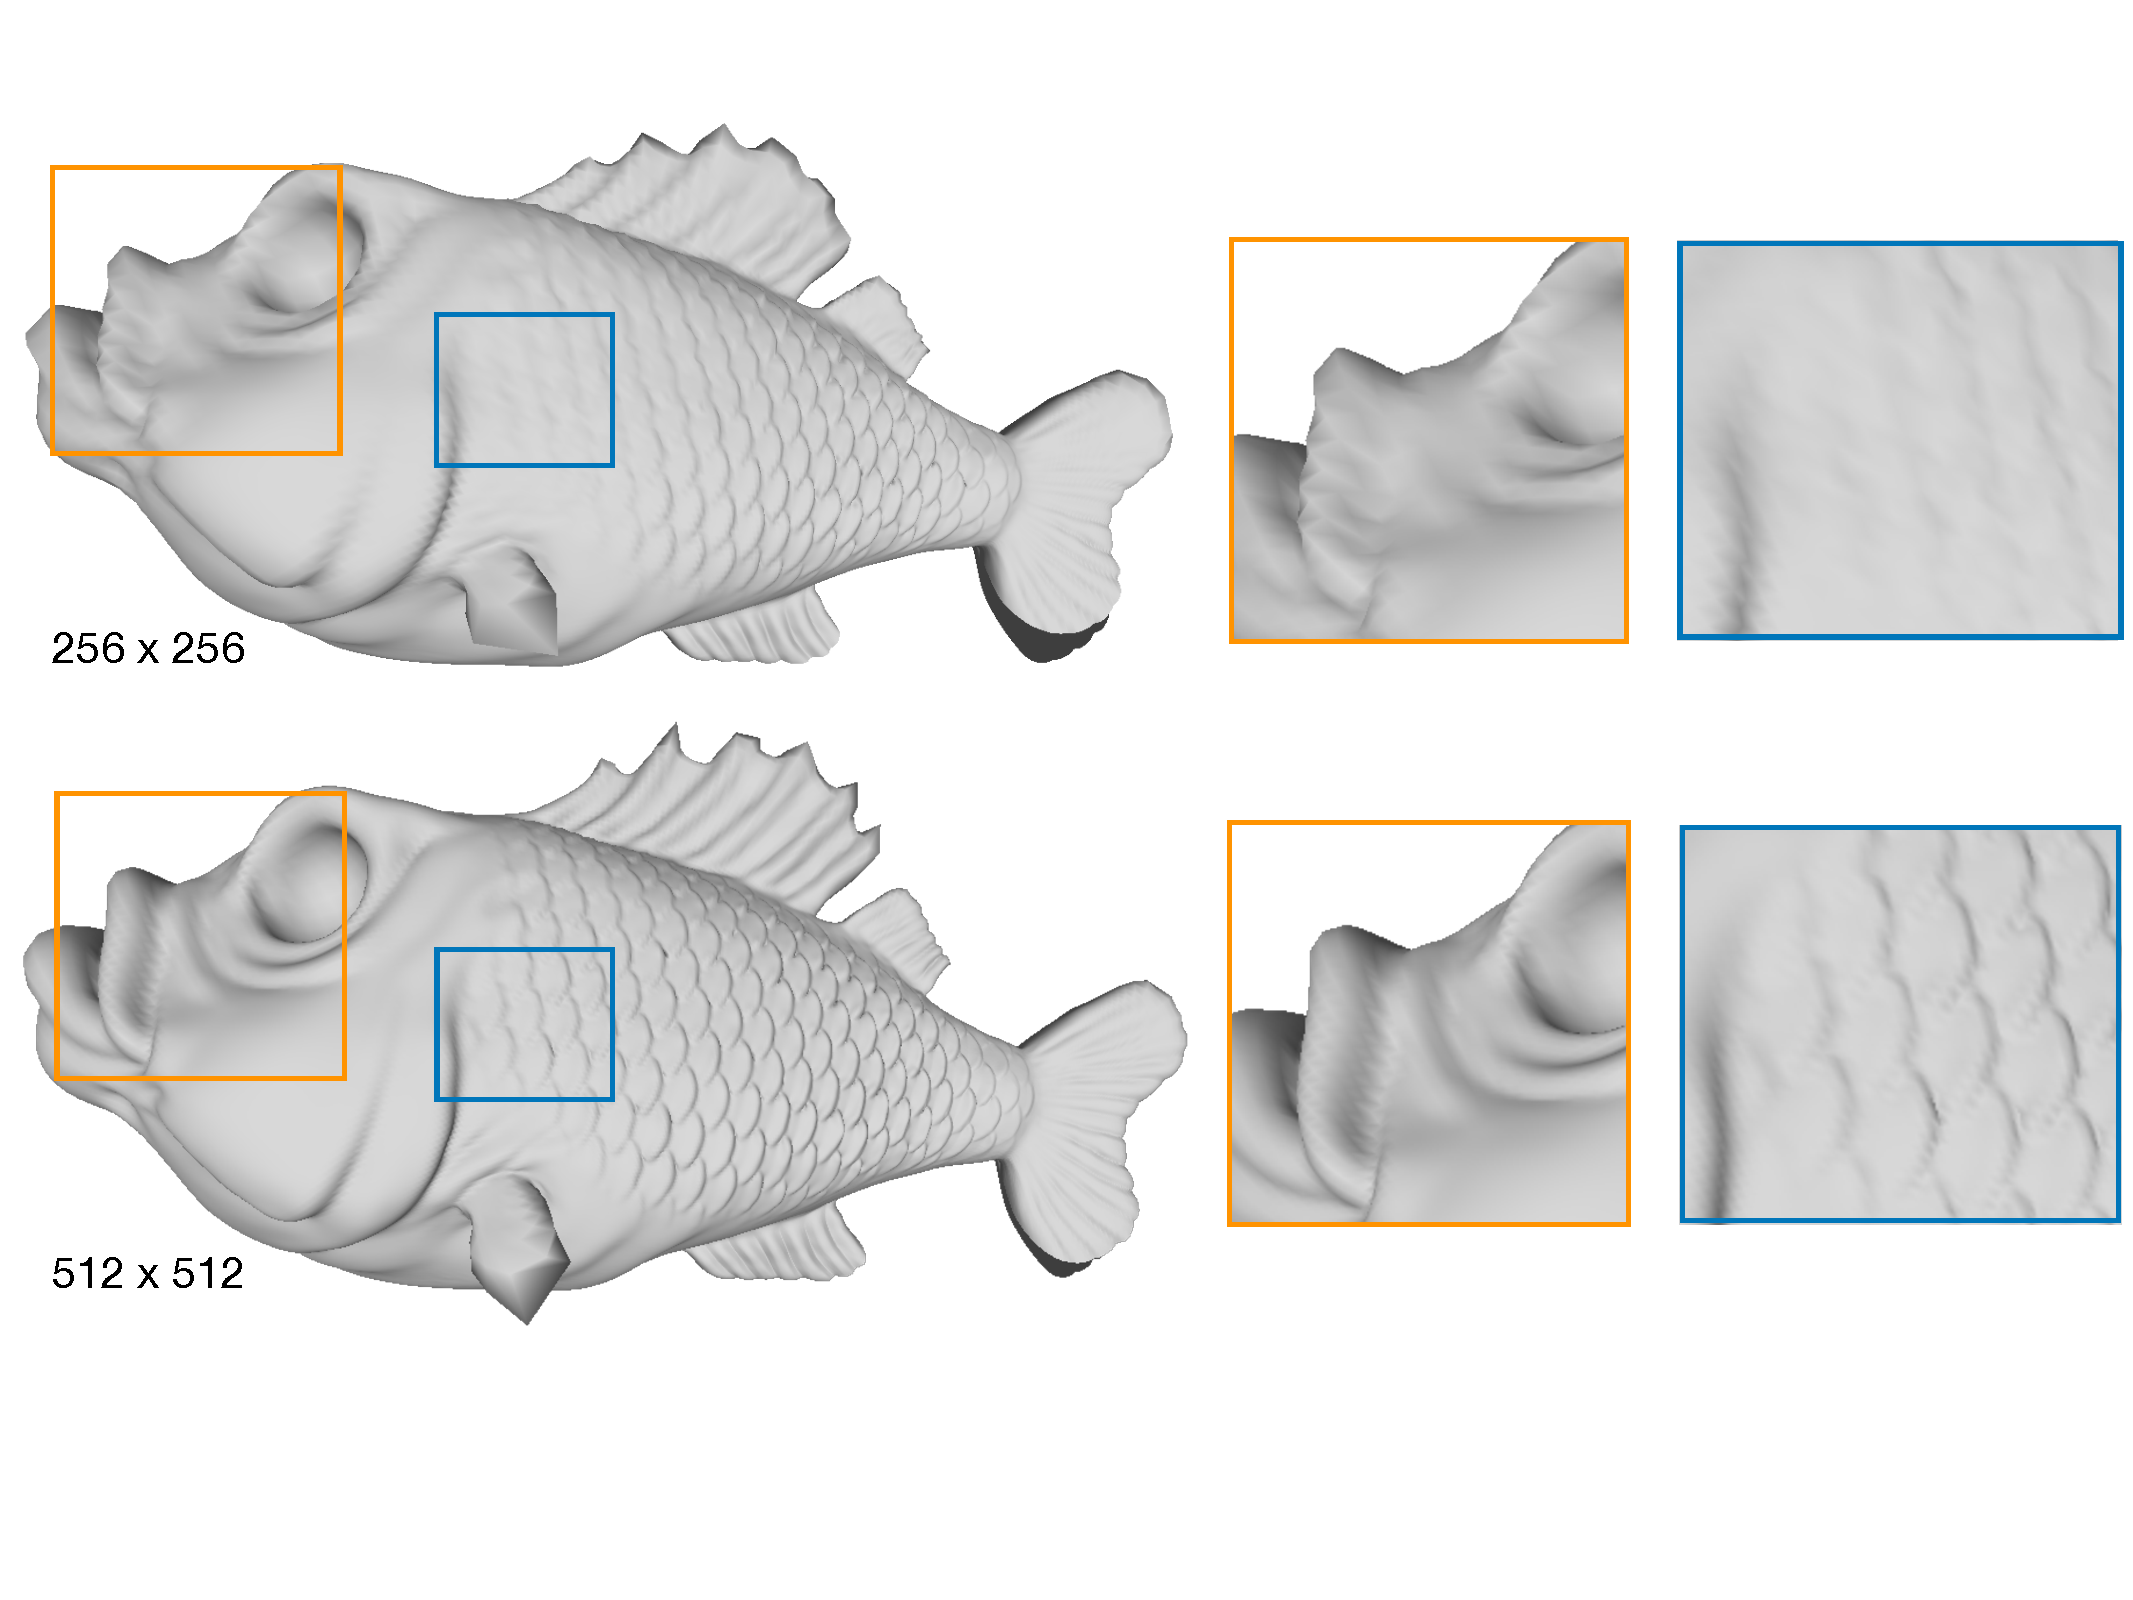
\includegraphics[width=0.4\textwidth]{Figures/fish}
     \caption{Fish reconstructions after uniform-resampling of Harmonic Map}
     \label{Fig: Fish Reconstruction}
\end{figure}~
This distortions arise due to the uniform remeshing, while using a sub-optimal choice of 2D surface parametrization (Harmonic Map), leading to poorly sampled surface areas in regions of higher curvatures. A more suited parametrization, that minimizes distortion after resampling, is the \textit{geometric-stretch} parametrization  \cite{gu2002geometry}.
%%%%%%%%%%%%%%%%%%%%%%%%%%%%%
% MEMORY and QUALITY
%%%%%%%%%%%%%%%%%%%%%%%%%%%%%
\subsection*{DeepPRT Quality and Memory Savings} \label{Sec: memory_savings}
For each of the test objects, our train- and validation sets together comprise 500 distinct object deformations. 
Within that deformation set, our U-Net model is able to achieve accuracies up to 98\% (table \ref{Table: NN_Accuracy}). Moreover, the resulting rendered appearances are close to indistinguishable from the ground truth. We further quantify the quality of the results using the perceptual metric SSIM, see Figure (\ref{Fig: DPRT_Quality}). 
\\
Based on this results, we imply that our trained network is able to faithfully approximate self-shadowing effects of 500 distinct shapes \textbf{at the very least}. Contrarily to classic PRT, which involves storing the transfer coefficients of each vertex for every single shape of the set, we only require the storage of the network parameters.
For our particular network of approx. $11,8$ million parameters,  the example objects with $256 \times 256$ and $512 \times 512$ number of vertices, and  a choice of $16$ transfer coefficients per vertex, this implies a compression ratio $r = (\text{\# PRT parameters})/(\text{\# network parameters})$ of: 
\begin{align*}
r_{diffuse} = 
\begin{cases}
\textbf{44.47 : 1} , & \mbox{for } 256^2 \mbox{ \#vertices} \\
\textbf{177.86 : 1} & \mbox{for } 512^2 \mbox{ \#vertices}
\end{cases}
\\
r_{glossy} = 
\begin{cases}
\textbf{133.41 : 1} , & \mbox{for } 256^2 \mbox{ \#vertices} \\
\textbf{533.56 : 1} & \mbox{for } 512^2 \mbox{ \#vertices}
\end{cases}
\end{align*}
for diffuse and glossy surfaces respectively.\\
This numbers grow linearly with an increasing number of coefficients, deformations or number of vertices. 
%%%%% TABLE %%%%%%%%%%%
\begin{table}[h]
\begin{tabular}{|l|l|l|l|l|}
\hline
\textbf{}            & \textbf{Accuracy} & \textbf{Train-Loss} & \textbf{Val-Loss} & \multicolumn{1}{c|}{\textbf{SSIM}} \\ \hline
\textbf{Pirate} & 0.9817            & 0.000397            & 0.000399                 & 0.99386                      \\ \hline
\textbf{Fish}        & 0.9729            & 0.002104            & 0.002200                      &  0.92451                   \\ \hline
\textbf{Cloth}       & 0.9818            & 0.000078            & 0.000098                 & 0.98840                      \\ \hline
\end{tabular}
\caption{Network Accuracy}
\label{Table: NN_Accuracy}
\end{table}
%%%%%%%%%%%%%%%%%%%
The numbers shown above express the compression ratio taking into account solely the training set. On top of that, our network shows good generalisation properties, also enabling accurate and qualitatively precise appearance predictions of deformations outside the training set. Thus, by taking this into account the compression ratio grows to immeasurable values. 
\\
Thus, we show that DeepPRT, as it is, is capable of drastically diminishing the storage consumption of PRT algorithms for deforming objects. 
\\
Last but not least, as mentioned above, deep convolutional networks itself can be highly optimised, hence making DeepPRT even much more efficient, energy, speed and memory wise \cite{Survey_NN_Compression}. 
%%%%%%%%%%%%%%%%%%%%%%%%%%%%%
% Comparisson 
%%%%%%%%%%%%%%%%%%%%%%%%%%%%%
\subsection*{Generality of DeepPRT and Comparison}
\subsubsection*{Generalisation Capability:}
We validate the generalisation capabilities of our model by standard machine learning procedures. We base our parameter tuning on minimising the validation loss and later analyse prediction quality using a test set.\\ 
The results show small errors and are in most cases visually indistinguishable or close to the ground truth (Figure [??]). 
\begin{figure}[H]
  \centering
    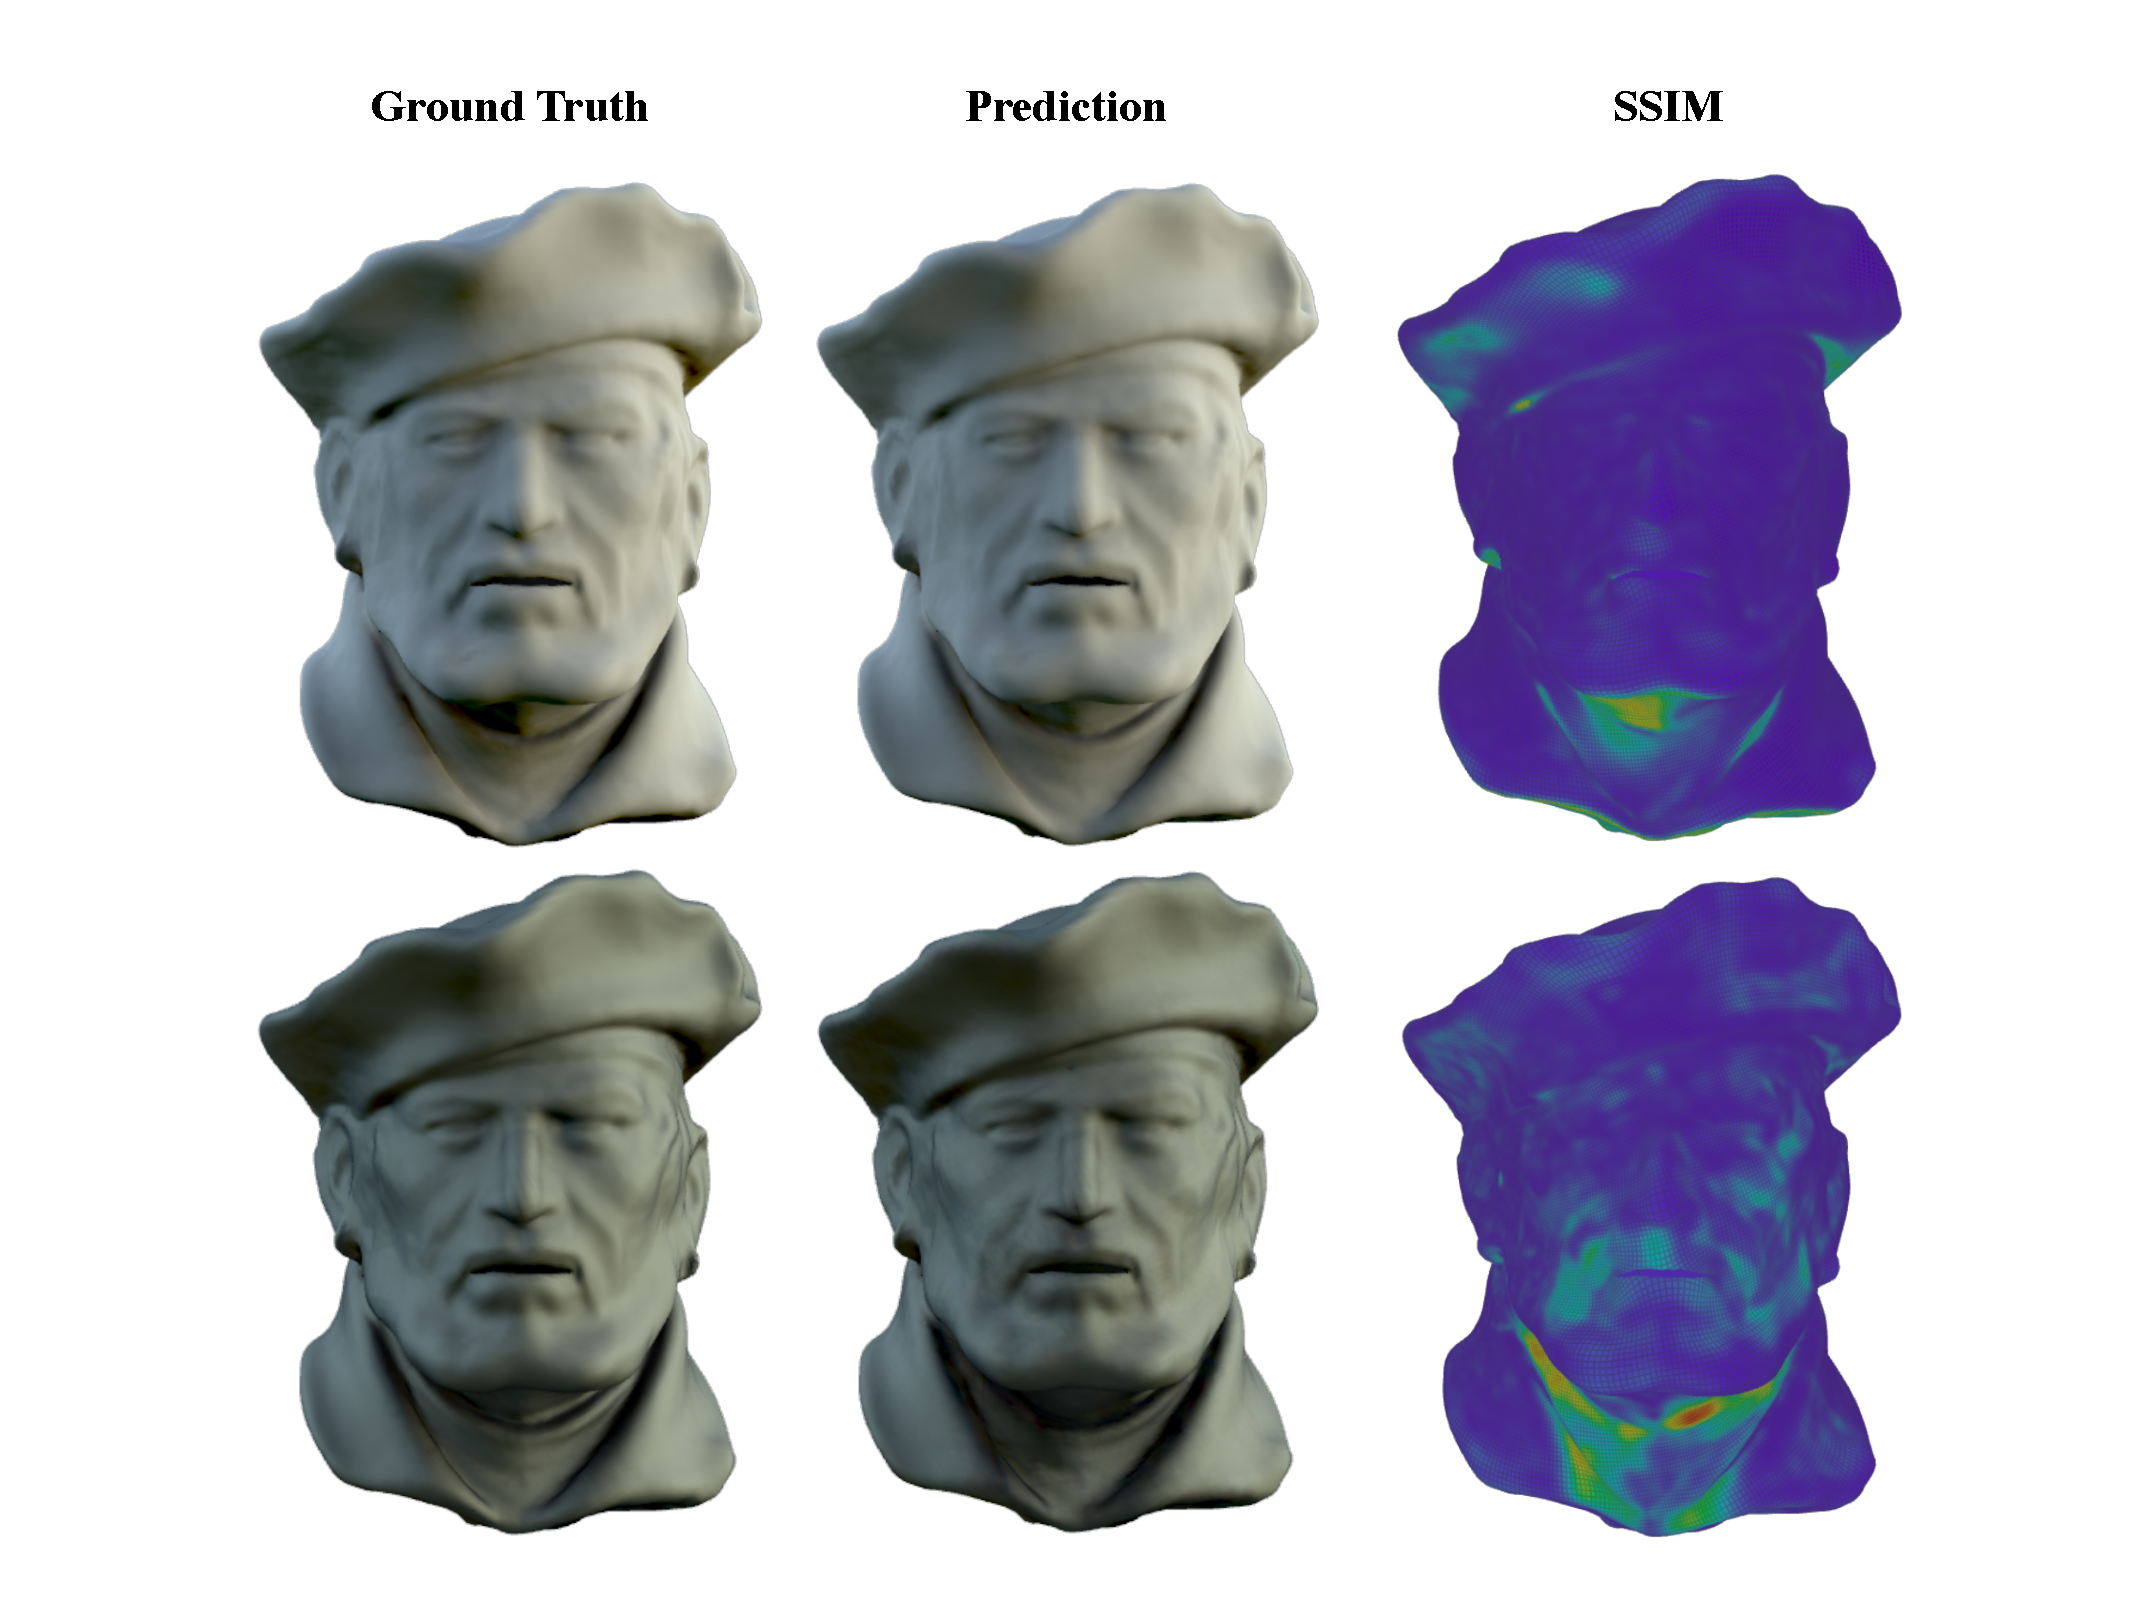
\includegraphics[width=0.35\textwidth]{Figures/glossy_pirate.pdf}
     \caption{Example: glossy pirate}
     \label{Fig: glossy_pirate}
\end{figure}
\subsubsection*{\textbf{Comparison with MoMoPRT}~:}
Furthermore, we compare our method with \cite{MoMoPRT} (MoMoPRT) and show that DeepPRT it is more accurate and can handle more general deformations. \\
The authors of \cite{MoMoPRT} proposed a linear model $f_{lin}$ to predict transfer coefficients within a "linear shape space", namely the space spanned by a Morphable Model.\\
This approach is clearly limited to shape deformations that are contained within the space described by the linear-shape-model $S_{lin}$ of choice. Moreover, although a linear model may be enough to approximate self-shadowing effects of shapes that are close to the mean shape of the training-data-distribution, the model lacks complexity to accurately approximate data samples that exist farther away from the mean shape (underfitting).  
\\
On the other hand, our more complex non-linear CNN model ($f_{CNN}$) is able to capture the relationships between the dataset's features (shape) and the target variable (transfer coefficients), enabling accurate approximations for a much larger deformation domain.\\
\\
For demonstration purposes, we generate a new training set consisting of, randomly sampled, linear combinations between visually more dissimilar basis shapes\footnote{More distinguishable between each other, than between each face expressions used in \cite{MoMo}.}: 1) the \textit{Pirate Head } on one side, and 2)  a simple \textit{Plane} on the other. We train both models, $f_{CNN}$ and $f_{lin}$, and compute their predictions for a series of test-shapes that are evenly distributed over the linear shape space. Figure (\ref{Fig:DPRT vs MoMoPRT A}) shows that the prediction accuracy of our $f_{CNN}$ model is higher and remains almost constant over the entire domain; on the contrary, the prediction accuracy of the linear model $f_{lin}$ drops significantly moving away from the mean shape (the \textit{Pirate/Plane} hybrid), as expected. 
\begin{figure}[h]
  \centering
    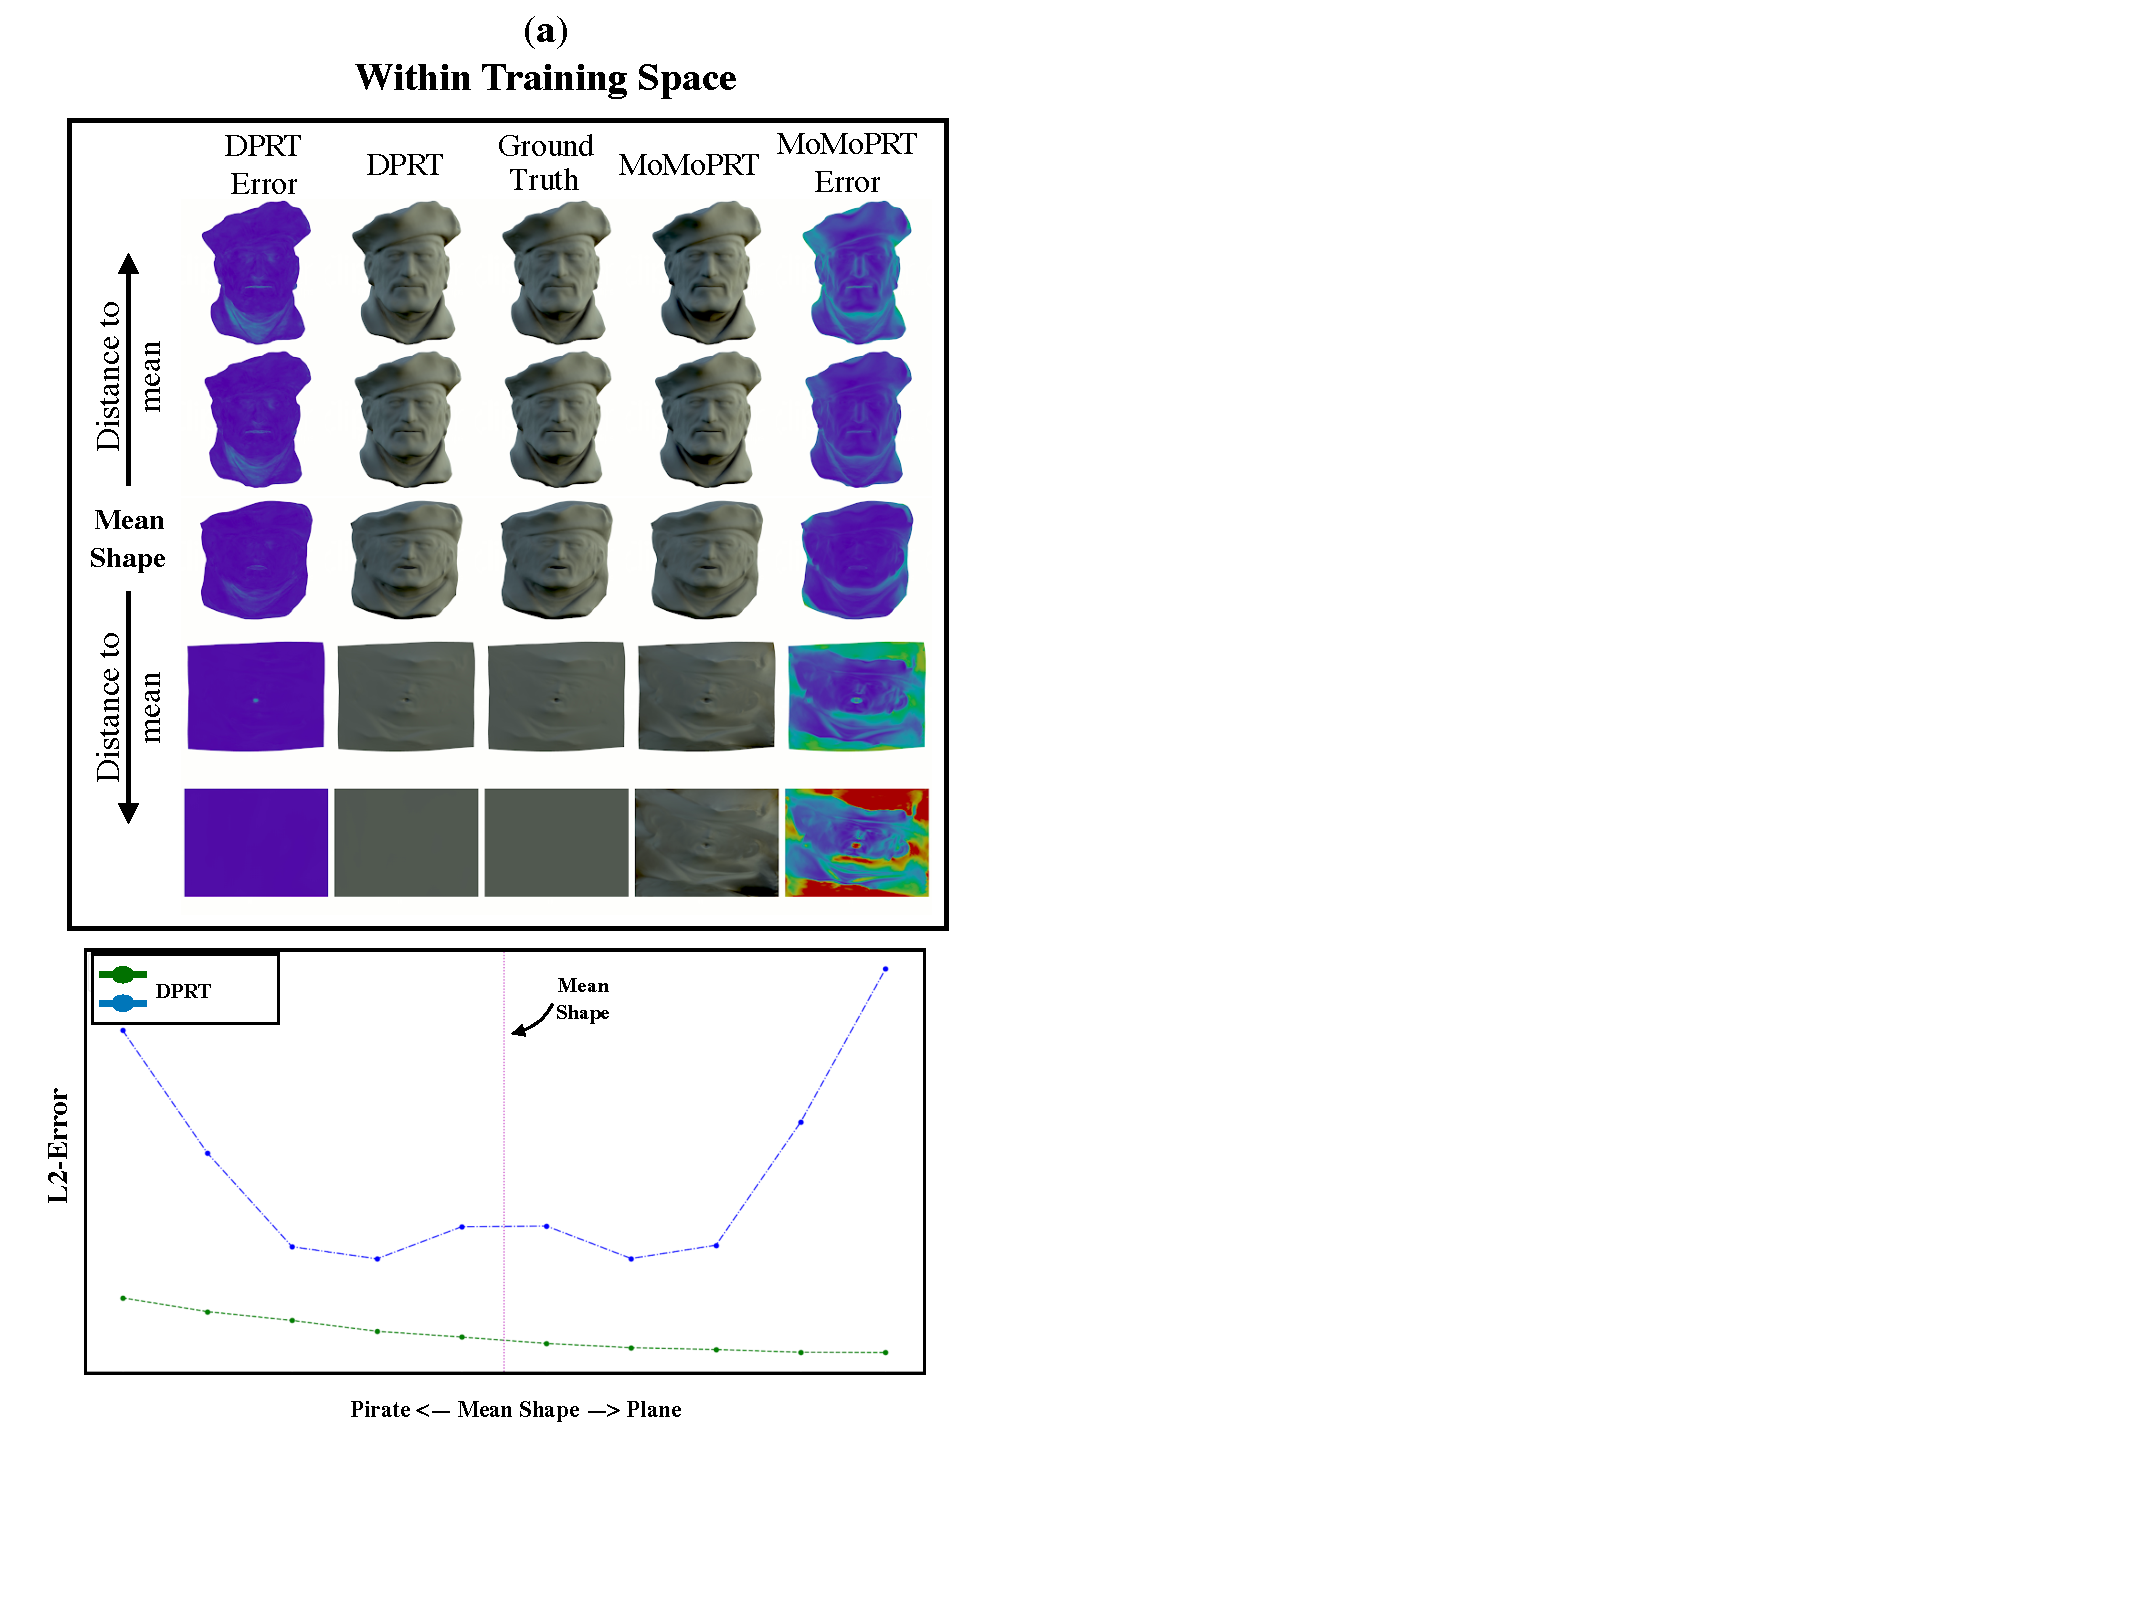
\includegraphics[width=0.4\textwidth]{Figures/DPRT_vs_MoMoPRT_a.pdf}
     \caption{Example: DPRT vs MoMoPRT}
     \label{Fig:DPRT vs MoMoPRT A}
\end{figure}
Last but not least, we demonstrate that our model approximates data that is contained in a much larger domain than the one spanned by a linear-shape-model $S_{lin}$. The models, $f_{CNN}$ and $f_{lin}$, are fed with a series of sample shapes, starting from the mean shape and increasingly deforming towards a \textit{Pirate} face expression that was excluded from the training set. \\
As can be seen in Figure (\ref{Fig:DPRT vs MoMoPRT B}), the linear model is not able to predict shapes away from its shape-space $S_{lin}$, while our method, again shows a close to constant prediction accuracy.
\begin{figure}[h]
  \centering
    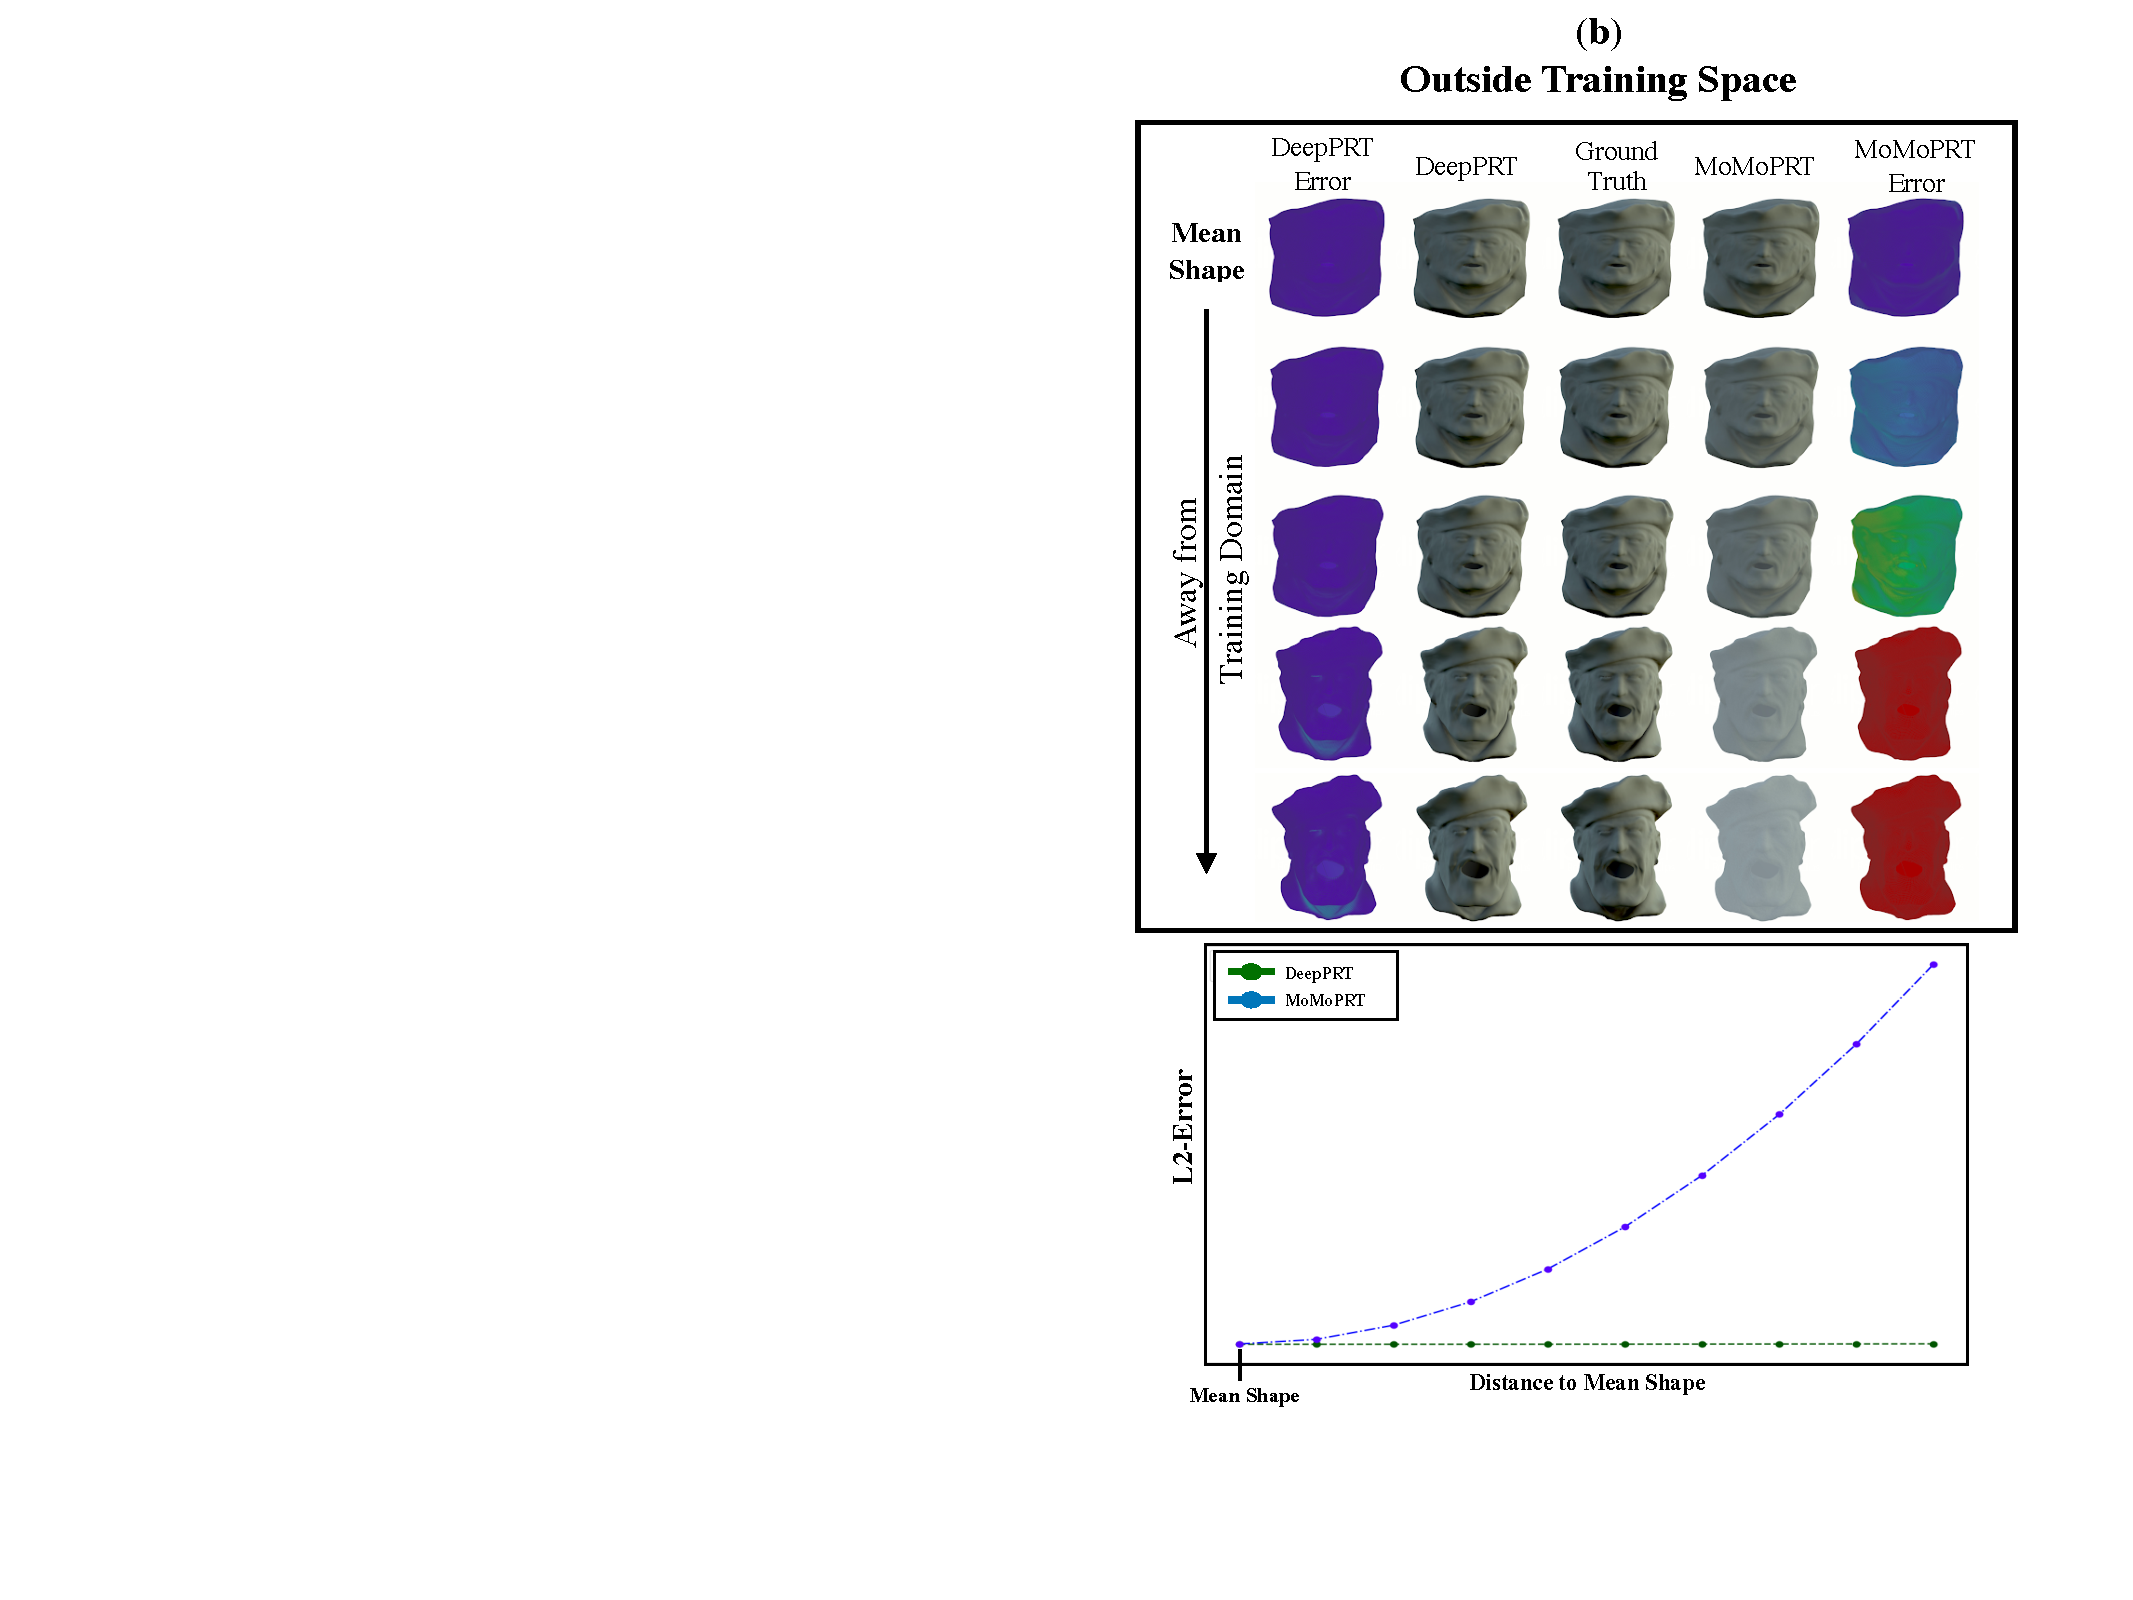
\includegraphics[width=0.4\textwidth]{Figures/DPRT_vs_MoMoPRT_b.pdf}
     \caption{Example: DPRT vs MoMoPRT}
     \label{Fig:DPRT vs MoMoPRT B}
\end{figure}

